\begin{figure}
    \centering
    \begin{subfigure}{0.48\textwidth}
        \centering
        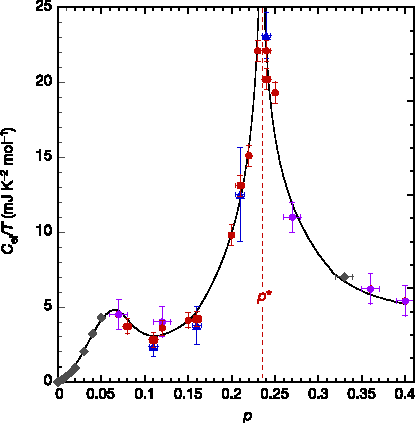
\includegraphics[width=\textwidth]{figures/michon}
        \caption{Measurements of Michon et al. showing a peak in $C/T$ which signifies the existence
            of a QCP.}
        \label{fig:michon}
    \end{subfigure}\hfill
    \begin{subfigure}{0.48\textwidth}
        \centering
        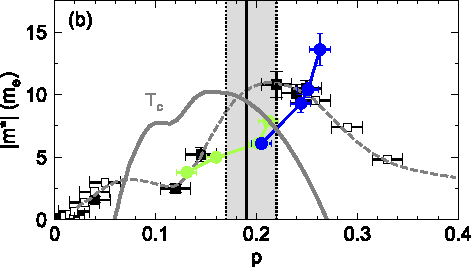
\includegraphics[width=\textwidth]{figures/legros}
        \caption{Measurements of Legros et al. drawn onto the measurements from Michon et al.,
            showing no peak in the cyclotron mass.}
        \label{fig:michon}
    \end{subfigure}
    \caption{Comparison of the measurements of Michon et al. and Legros et al.}
    \label{fig:comparison}
\end{figure}

\subsection{Evidence against the QCP: Optical Conductivity}
In their 2022 paper, Legros et al. \cite{legros2022} instead used optical conductivity to
probe the QCP. To do so, the first measured the optical conductivity of LSCO cuprates in various
fields. Then, they fitted a model for the conductivity called the Drude formula to the data. The
Drude formula is a simple classical model that has been used for a long time in condensed matter
physics to model conductivity. Next, they extracted the cyclotron mass from the parameters of the
fit. Finally, they extracted the cyclotron mass from the parameters of the fit. To do so, they
calculated the cyclotron frequency in different magnetic fields and found the mass by fitting a
linear relation between the cyclotron frequency and the magnetic field;
\begin{equation}
    \omega_c = \frac{eB}{m_c}.
\end{equation}
They argue the cyclotron mass is the same as the effective mass of the charge carriers
($m_c \sim m^*$).

At the end of all the analysis, Legros et al. found that the cyclotron mass does not peak
at the critical doping level and simply increases with doping. This is in contradiction with the
results of Michon et al. and suggests that there is no QCP in Cuprates.

We believe, however, that their data analysis is problematic, because of the use of the Drude
formula. Eventhough the Drude formula is derived using classical physics, it is highly effective for
analysing the conductivity of materials, which emerges from the collective quantum behavior of the
electrons. But, this is only the case when the material has roughly isotropic electronic properties
(more precisely, the Fermi surface needs to be approximately isotropic). This is not true for
Cuprates, which have highly anisotropic electronic properties. Also, the effective mass of the
charge carriers is not necessarily the same as the cyclotron mass, but we only focus on the former
issue in this project.
